\chapter{IT-Sicherheitsmanagement für vernetzte Systeme}
Zusammenfassung der Vorlesung  "`IT-Sicherheit für vernetzte Systeme"' von Professor Hartenstein aus dem Wintersemester 2013.\footnote{\url{http://dsn.tm.kit.edu/pastcourses_3385.php}}

\section{Einführung}

\subsection{Management}
"`Bezeichnung einerseits für die Führung von Institutionen jedweder Art andererseits für die Gesamtheit der Personen, die diese Funktion erfüllen."'\footnote{Brockhaus-Enzyklopädie in 24 Bänden, 19. Aufl., Band 14, 1991}

\subsubsection{Handlungsorientiertes Managementkonzept}
Prozesse der Entscheidungsfindung und Entscheidungsdurchsetzung.
\begin{itemize}
	\item Gesamtheit der Handlungen
	\item Bestmögliches Erreichen der Ziele einer Institution
	\item Auf die beteiligten Interessensgruppen gerichtet
	\item \textbf{Strukturierung in Aufgabenbereiche}
	\begin{itemize}
		\item Grundsatz- und Zielbildung
		\item Planung
		\item Organisation
		\item Kontrolle
	\end{itemize}
\end{itemize}

\subsubsection{Personenorientiertes Managementkonzept}
Fokus liegt auf den Aufgaben sowie den Befugnissen und Aufsicht/Kontrolle der handelnden Personen.\\
Die Personengruppen sind durch Gesetze, Satzungen oder Aufträgen mit Rechten, Pflichten und Verantwortung ausgestattet.

\subsubsection{Handhabungssorientiertes Managementkonzept}
\begin{itemize}
	\item Management-Techniken und Methoden
	\item Qualitativer und quantitativer Art
	\item Prognose-, Planungs- und Entscheidungstechniken
	\item Einbeziehung/Basis von Managementinformationssystemen
\end{itemize}


\subsection{IT-Sicherheitsmanagement}
\begin{itemize}
	\item Allumfassender Ansatz
	\item Ziel: Angemessenes Sicherheitsniveau
	\item Verlangt: Abschätzung des Risikos
	\item Immerwährender Prozess: Planung/Organisation - Umsetzung/Durchsetzung - Aufrechterhaltung und Erfolgskontrolle
\end{itemize}

\subsubsection{Informationssicherheit}
\begin{itemize}
	\item Hauptaspekte: Vertraulichkeit, Verfügbarkeit und Integrität zum Erhalt eines kontinuierlichen Geschäftsbetriebs\footnote{\url{http://standards.iso.org/ittf/PubliclyAvailableStandards/c041933_ISO_IEC_27000_2009.zip}}
	\item Umsetzung eines geeigneten Maßnahmenkatalogs
	\item Festgelegter Risikomanegementprozess
	\item Umsetzung mit Hilfe eines ISMS
	\item Die Maßnahmen müssen festgelegt, umgesetzt, überwacht, überprüft und verbessert werden
	\item Ziel: Erreichen des spezifischen Unternehmenssicherheitsniveaus
\end{itemize}


\subsection{IT-Sicherheitsmanagement: Prinzipien}

\subsubsection{Prinzipien: Die 6 Ps}
Siehe handlungsorientiertes Management.
\begin{itemize}
	\item Richtlinien (Policy)
	\item Planung (Planning)
	\item Programme (Programs)
	\item Schutzmaßnahmen (Protection)
	\item Menschen (People)
	\item Projektmanegement
\end{itemize}

\subsection{Strukturierung der Vorlesung}
\begin{itemize}
	\item Konzepte
	\item Standards
	\item Vorgehensweisen
	\item Fallstudien und -beispiele
\end{itemize}



\section{Bedrohungsszenarien und IT-Schutzziele}

\subsection{Potentielle Bedrohungen und Angreifer}

\subsubsection{Klassifizierung und Angreifer}
\begin{itemize}
	\item Zielsetzung (Wann ist der Angriff ein Erfolg?)
	\item Fokussierung (Muss ein bestimmtes Ziel angegriffen werden?)
	\item Ressourcen (Welche Ressourcen stehen dem Angreifer zur Verfügung?)
	\item Motivationsstärke (Wie wichtig ist dem Angreifer das Erreichen der Zielsetzung?)
\end{itemize}

\subsubsection{Typische Zielsetzungen eines Angreifers}
\begin{itemize}
	\item Zugriff auf Ressourcen
	\item Zugriff auf Informationen
	\item Manipulation eines Dienstes
	\item Sabotage
\end{itemize}

\subsubsection{Ressourcen des Angreifers}
\begin{itemize}
	\item Personelle Ressourcen
	\item Finanzielle Ressourcen
	\item Technische Ressourcen
	\item Insiderwissen
	\item Einfluss auf das Ziel
\end{itemize}

\subsubsection{Motivationsstärke des Angreifers}
\begin{itemize}
	\item Persönliche, nicht-finanzielle Interessen: Ansehen, politische Überzeugung, Interesse. Sicherheitsmaßnahmen so weit erhöhen, dass der Angriff aufwendig wird
	\item Finanzieller Gewinn: Rentabilität. Sicherheit so weit erhöhen, dass der Angriff unrentabel wird
	\item Politisches oder strategisches Ziel: Sicherheit muss so weit erhöht werden, dass Angriff unmöglich ist (praktisch kaum zu bewältigen)
\end{itemize}

Angriffe können gezielt oder ungezielt sein. Für einen gezielten Angriff ist ein höheres Sicherheitsniveau erforderlich. (Anderenfalls muss man nur besser sein als die anderen.)

\subsubsection{Beispiele von Angreifern}
\begin{itemize}
	\item Staatliche Institutionen: Informationen oder Sabotage
	\item Gezielte Hacker-Angriffe: Manipulation von Diensten. Bsp: Drogenschmuggel mit Ausspähen von Häfen.
	\item Ungezielte Hacker-Angriffe: Meist Zugriff auf Informationen oder Ressourcen
	\item Gelegenheitsangriffe
\end{itemize}


\subsection{Schutzziele der IT-Sicherheit}

\subsubsection{IT-Sicherheit / Informationssicherheit}
Schützen von Informationen bzw. Daten einschließlich zugehöriger Komponenten wie etwa der Systeme und Hardware, die diese Information nutzt, speichert oder überträgt.\\
Differenzierung zur allgemeinen Sicherheit erfolgt über die sogenannten Schutzziele.

\subsubsection{Schutzziele}

Die klassischen Triaden: Confidentiality, Integrity, Availability (CIA).

\begin{itemize}
	\item Authentizität: Echtheit und Glaubwürdigkeit eines Objekts (Übergeordnetes Schutzziel)
	\item Vertraulichkeit: Keine unautorisierte Informationsgewinnung
	\item Integrität: Keine Möglichkeit, Daten unautorisiert zu manipulieren
	\item Verfügbarkeit (Abgrenzung gegenüber Robustheit)
	\item Datenschutz
	\item Anonymität und Pseudonymität
	\item Verbindlichkeit
\end{itemize}



\section{Der IT-Sicherheitsprozess}

\subsection{Was ist ein IT-Sicherheitsprozess?}

Ergänzung der Schutzziele durch Richtlinien und Gesetze, Sicherheitsbewusstsein, Schulungen, Planung und Organisation.

\begin{itemize}
	\item Was ist ein angemessenes Sicherheitsniveau?
	\item Welche Ressourcen müssen geschützt werden?
	\item Wie werden die Ressourcen geschützt?
\end{itemize}

\subsubsection{Umsetzung von IT-Sicherheit}
\begin{itemize}
	\item Zugangs- und Zugriffskontrolle
	\item Kryptokonzept und Monitoring
	\item Redundanz, Backup und Archivierung
	\item Patches und Upgrades
	\item Firewalls, Intrusion Detection und Intrusion Prevention
\end{itemize}

\subsubsection{Klassisches Prozessmodell: Wasserfall-Modell}
\begin{enumerate}
	\item Voruntersuchung
	\item Analyse
	\item Grobentwurf
	\item Feinentwurf
	\item Realisierung
	\item Betrieb und Wartung
\end{enumerate}
Jeweils nur ein Sprung zum Vorgänger bzw. Nachfolger möglich.

\subsubsection{Inkrementelles Modell}
\begin{itemize}
	\item Voruntersuchung/Analyse
	\item Definition
	\item Entwurf
	\item Realisierung
	\item Betrieb
\end{itemize}
Inkrementelles Modell, daher nach \textit{Betrieb} ein Sprung zu \textit{Definition}.

\subsubsection{Spirallmodell}
Die Spirale besteht aus den folgenden Teilschritten, die jeweils immer wieder abgearbeitet werden und weiter nach außen gehen.
\begin{itemize}
	\item Analyse, Identifikation der Ziele
	\item Evaluierung der Alternativen, Risikoanalyse
	\item Entwicklung und Verifikation (Wasserfallmodell, inkr. Modell, etc.)
	\item Planung der nächsten Schritte, Überprüfung
\end{itemize}

\subsection{Internationale Umsetzung: ISO 2700x}

\begin{itemize}
	\item Ziel: Normierung des IT-Sicherheitsprozesses, Katalog von "`Best Practise"'-Vorschlägen, detaillierte Behandlung ausgewählter Problemfelder (z.B. Risikoanalyse), Grundlage für Zertifizierung
	\item Aber: Kein Anspruch auf Vollständigkeit!
\end{itemize}

\subsubsection{ISO 27000: Informationssicherheits-Managementsystem (ISMS)}
\begin{itemize}
	\item Ganzheitlicher Prozess
	\item Risikoanalyse
	\item Risikoakzeptanz (Risiko vs. Kosten)
	\item Risikomanagement (aktive Prävention und Neubewertung)
\end{itemize}

\subsubsection{ISO 27001: Prozessmodell}
\begin{itemize}
	\item Planen: Definition des Anwendungsbereichs und der Sicherheitsleitlinie, Organisation der Risikoanalyse, Auswahl von Maßnahmen, Koordination mit Management
	\item Durchführen (Do): Risikobehandlung und Umsetzung der Maßnahmen, Schulungen und Bewusstseinsbindung
	\item Prüfen (Check); Überwachung der Maßnahmen, Prüfen der Wirksamkeit, Überprüfung der Risikoeinschätzung, interne Befragungen (Audits)
	\item Handeln (Act): Umsetzung identifizierter Verbesserungen, Verbeugung neuer Risiken, Sicherstellen, dass die Verbesserungen ihre Ziele erreichen
\end{itemize}

\subsubsection{Verantwortung des Managements}
\begin{itemize}
	\item Zielbildung: Festlegung der Sicherheitsleitlinie und des Sicherheitsniveaus
	\item Organisation: Bestimmung von Verantwortlichkeiten, Bereitstellung der Ressourcen
	\item Schulung und Bewusstseinsbildung
	\item Kontrolle: Regelmäßige Überprüfung, Analyse und Bewertung
\end{itemize}

\subsubsection{ISO 27002: Sicherheitsleitlinie}
Verbindliche Grundsätze für die IT-Sicherheit.
\begin{itemize}
	\item Bedeutung der Sicherheit definieren, Absicht des Managements erklären
	\item Zielsetzung
	\item Strategie: Rahmen für Risikoeinschätzung und Risikomanegement, Berücksichtigung gesetzlicher und vertraglicher Anforderungen
	\item Organisation: Verantwortlichkeiten festlegen, Verweise auf weiterführende Dokumente
\end{itemize}

\subsubsection{Aufbau und Struktur am Beispiel des KIT}
\begin{itemize}
	\item Präambel
	\item Geltungsbereich
	\item Zielsetzung
	\item Organisation
	\item IT-Sicherheitsprozess am KIT
	\item Sachverwandte Themen
\end{itemize}
Knapp formuliert (5 Seiten).

\subsubsection{Maßnahmen zur Behandlung identifizierter Risiken}
\begin{itemize}
	\item Behandlung mittels Maßnahme (Risikoreduktion)
	\item Tolerierung des Risikos (Restrisiko)
	\item Vermeidung/Eleminierung spezieller Risiken
	\item Übertragung des Risikos auf Dritte (z.B. Versicherung)
\end{itemize}


\subsection{Deutsche Umsetzung: BSI-Grundschutz}
\begin{itemize}
	\item Empfehlungen von Standardsicherheitsmaßnahmen für typische IT-Systeme
	\item Organisatorische, personelle, infrastrukturelle und technische Standardsicherheitsmaßnahmen
	\item Baukastenprinzip
	\item Gefährdungs- und Maßnahmenkataloge
	\item Werkzeugunterstützung
	\item Bedarfsgerechte Weiterentwicklung (...aber leider etwas zu langsam)
\end{itemize}

\subsubsection{IT-Sicherheitsprozess nach BSI GSK}
\begin{itemize}
	\item Strategische Ebene: Initiierung, Erstellung der Sicherheitsleitlinie, Einrichtung des IT-Sicherheitsmanagements
	\item Taktische Ebene: Erstellung eines IT-Sicherheitskonzepts
	\item Operative Ebene: Umsetzung und Aufrechterhaltung im laufenden Betrieb
\end{itemize}

\subsubsection{Entwicklung eines IT Sicherheitskonzepts nach GSK}
\begin{enumerate}
	\item IT-Strukturanalyse: Ermittlung des zu schützenden IT-Verbunds
	\item Schutzbedarfsfeststellung
	\item IT-Grundschutzanalyse: Modellierung über Baukastensystem und Basissicherheitscheck
	\item Ergänzende Sicherheitsanalyse (bei hohem Schutzbedarf): Risikoanalyse, Penetrationstest, Differenz-Sicherheitsanalyse (etablierte Musterlösungen hochschutzbedürftiger Systeme)
	\item Realisierungsplanung
\end{enumerate}

\subsubsection{Schutzbedarfsfeststellung}
\begin{itemize}
	\item Klassisches Vorgehen: Ermittlung der bedrohten Objekte und Bedrohungen, dann Risikoanalyse
	\item GSK vereinfacht: Pauschale Schutzbedarfsfeststellung über die Schadensauswirkungen
	\item Schutzbedarfsfeststellung für \textit{jedes} Schutzziel separat
	\item Mögliche Prinzipien: Maximumsprinzip (Schutzbedarf orientiert sich am höchsten Schadenspotential), Kumulationseffekt (Schutzbedarf des Systems ist höher als Schutzbedarf aller Anwendungungen kumuliert), Verteilungseffekt (Invers zu Kumulationseffekt)
\end{itemize}

\subsubsection{Gefährdungskatalog}
\begin{itemize}
	\item Elementare Gefährdungen
	\item Höhere Gewalt
	\item Organisatorische Mängel
	\item Menschliche Fehlhandlung
	\item Technisches Versagen
	\item Versätzliche Handlungen
\end{itemize}

\subsubsection{Vergleich zu ISO 2700x}
\begin{itemize}
	\item BSI GSK konkretisiert das recht allgemeine ISO 2700x-Paket
	\item Vorteile: Detaillierter, Berücksichtigung deutscher Besonderheiten (Rechtslage, etc.)
	\item Nachteile: Grundschutz recht starr, BSI Maßnahmen oft zu konkret und nicht aktuell
	\item Fazit: Nur für mittelgroße IT-Verbunde geeignet, sonst "`Overkill"'
\end{itemize}



\section{Rechtliche Anforderungen}

\subsection{Motivation}

\subsubsection{Fragen aus dem Betrieb}
\begin{itemize}
	\item Welche Gesetze sind einschlägig?
	\item Welche (Log-)Daten darf ich speichern und wie lange?
	\item Welche Schutzmaßnahmen sind vorgeschrieben?
\end{itemize}

\subsubsection{Mögliche Gesetze}
\begin{itemize}
	\item Bundesdatenschutzgesetz
	\item Telemediengesetz und Telekommunikationsgesetz
	\item Kreditwesengesetz, HGB und KonTraG
	\item Signaturgesetz
\end{itemize}

\subsubsection{Herausforderungen bei der IT-Compliance}
\begin{itemize}
	\item Vollständigkeit nur schwer erreichbar
	\item Abwägung unterschiedlicher Anforderungen nötig
	\item Die Abgrenzung von Regelungsbereichen (Wechselwirkung von verschiedenen Gesetzen) ist zu beachten
	\item Gewichtung und Angemessenheit muss gewahrt werden
\end{itemize}

\subsection{Abgrenzung von Regelungsbereichen}
Die Abgrenzung von Regelungsbereichen, d.h. die Wechselwirkung von verschiedenen Gesetzen ist zu beachten.\\
Beispiel: Welche Regelungsbereiche sind für den Bereich elektronischer Kommunikationsnetzen und -diensten einschlägig?\\
Abgrenzung/Zuordnung in der Praxis oft umstritten.\\

\subsubsection{Exemplarische Abgrenzung: Ebenen der Kommunikation}

\begin{tabularx}{\columnwidth}{|X|X|l}
	\hline
	\textbf{Inhaltsebene}: z.B. Abwicklung von Bankgeschäften, Versandhandel & \textbf{Offline-Recht}: Bundesdatenschutzgesetz, Bereichsspezifische Gesetze \\
	\hline
	\textbf{Interaktionsebene}: Teledienste und Mediendienste & \textbf{Online-Recht}: Telemediengesetz \\
	\hline
	\textbf{Transportebene}: Telekommunikationsdienste & \textbf{Telekommunikationsrecht}: Telekommunikationsgesetz \\
	\hline
\end{tabularx}

\subsubsection{Telekommunikationsgesetz}
\begin{itemize}
	\item Fernmeldegeheimnis
	\item Datenschutz
	\item TK-Überwachung und Vorratsdatenspeicherung
	\item Nicht verantwortlich für den Inhalt
	\item Sicherheitskonzept notwendig, wenn TK-Anlagen betrieben werden
\end{itemize}

\subsubsection{Telemediengesetz}
\begin{itemize}
	\item Datenschutz
	\item Impressumspflicht
	\item Regelmäßig verantwortlich für den Inhalt
\end{itemize}


\subsection{Datenschutz}
Schutz von personenbezogener Daten\footnote{Bundesdatenschutzgesetz}. Datensicherheit ist meistens vorausgesetzt, bzw. notwendig.

\subsubsection{Unterscheidung zwischen 3 Phasen}
\begin{itemize}
	\item Erhebung
	\item Verarbeitung, Speicherung, Übermittlung
	\item Nutzung
\end{itemize}

\subsubsection{Grundsätze des BDSG}
\begin{itemize}
	\item Präventives Verbot mit Erlaubnisvorbehalt
	\item Zweckbindungsgebot
	\item Transparenzgebot: Auskunftspflicht und Berichtspflicht
	\item Gebot Verhältnismäßigkeit, Datenvermeidung und Datensparsamkeit
	\item Technische und organisatorische Schutzmaßnahmen
\end{itemize}


\subsection{Aufsichtsrechtliche Regelungen für IT-Finanzdienstleister}

\subsubsection{MaRisk}
\begin{itemize}
	\item Abgeleitet aus dem KWG
	\item Mindestanforderungen an das Risikomanagement
	\item Herausgegeben von der BaFin
	\item Präventiv ausgerichtet mit risikoorientiertem Aufsichtsprozess
	\item Verwendung von internat. und nat. Normen (ISO 2700x, BSI GSK)
	\item Vergleichbare Maßnahmen und vereinfachte Prüfung
	\item Auswirkungen auf die Software-Entwicklung: Programmierrichtlinie, Testverfahren, Funktionstrennung von Entwicklung und Abnahme/Test, Dokumentation und Versionierung
	\item Umfangreiches Notfallmanagement
\end{itemize}


\subsection{Aktuelles: Geplantes IT-Sicherheitsgesetz}

\subsubsection{Kernpunkten des Referentenentwurfs}
\begin{itemize}
	\item Pflicht zur Erfüllung von Mindeststandards
	\item Pflicht zur Meldung erheblicher Sicherheitsvorfälle
	\item Jährliche Berichtspflicht des BSI
\end{itemize}


\subsection{Zusammenfassung}
\begin{itemize}
	\item Zahlreiche Gesetze mit (in-)direktem Bezug zur IT-Sicherheit
	\item Datenschutz
	\item Regulierung im Finanzsektor durch KWG und MaRisk
	\item Weitere Regulierungen auf nat. und europäischer Ebene zu erwarten (z.B. IT-Sicherheitsgesetz)
\end{itemize}

\section{Risikoanalyse und -management}

\subsection{Motivation}
\begin{itemize}
	\item Risiken sind per se nichts Schlechtes
	\item Risiken müssen allerdings konsequent gemanagt werden
	\item "`Geht ein Unternehmen kein Risiko ein, wird es sofort von offensiveren Wettbewerbern überholt"'\footnote{Bärentango: Mit Risikomanagement Projekte zum Erfolg führen von Tom DeMarco}
\end{itemize}


\subsection{Risikomanagement}
\[Risiko = Eintrittswahrscheinlichkeit\cdot Schadenspotential\]

\subsubsection{Methoden der Risikoanalyse}
\begin{itemize}
	\item Qualitative Einstufung
	\item Quantitative Einstufung
\end{itemize}

Risikomanagement bildet eine fundierte Basis für Entscheidungen und dient somit als Steuerinstrument, um Ressourcen effektiv zu nutzen.\\
Die Vorgehensweise orientiert sich an Plan-Do-Check-Act.

\subsection{Spezifika des IT-Risikomanagement}
\begin{itemize}
	\item Risikomanagement bildet einen wesentlichen Baustein im IT-Sicherheitsmanagement
	\item Integration in das Risikomanagement des Unternehmens
	\item Definiert in ISO 27005
\end{itemize}

\subsubsection{ISO 27005: Der IT-Sicherheitsrisikoprozess}
\begin{enumerate}
	\item \textbf{Festlegung der Rahmenbedingungen}
	\begin{itemize}
		\item Methodik festlegen (ISO 27005 gibt nur den Rahmen vor)
		\item Evaluierungskriteren entwickeln
		\item Potentielle Auswirkungs(-kategorien) festlegen
		\item Fokus und Grenzen festlegen
		\item Organisation im Unternehmen (Rollen zuweisen, etc.)
	\end{itemize}
	\item \textbf{Risikoidentifizierung}
	\begin{itemize}
		\item Identifikation von Szenarien, die zu einem Schaden führen können
		\item Identifikation von Assets, Bedrohungen, umgesetzten Maßnahmen, Schwachstellen und potentielle Auwirkungen
	\end{itemize}
	\item \textbf{Risikoanalyse}
	\begin{itemize}
		\item Bestimmung des Schadenspotentials (z.B. durch statistische Daten)
		\item Bestimmung der Eintrittswahrscheinlichkeit
		\item Qualitative oder quantitative Bewertung möglich
	\end{itemize}
	\item \textbf{Risikobewertung}
	\begin{itemize}
		\item Priorisierung der Risiken auf Basis der Evaluationskriterien und Akzeptanzkriterien
		\item Ist kompetenzgerecht vorzunehmen
	\end{itemize}
	\item \textbf{Risikobehandlung}
	\begin{itemize}
		\item Mögliche Methoden zur Risikobehandlung s.o.
		\item Ggf. sind Maßnahmen vorzuehmen
		\item Entscheidungen kompetenzgerecht
	\end{itemize}
\end{enumerate}

Iterativer Prozess, daher im Anschluss ein Sprung zu (1).

\subsubsection{Qualitative vs. quantitativer IT-Risikobewertung}
\begin{itemize}
	\item Quantitativ: Hinterlegung von konkreten Werten
	\item Qualitativ: Konkrete Werte meist schwierig zu erlangen, daher Bewertung in Stufen (von Eintrittswahrscheinlichkeit und Schadenspotential $\rightarrow$ Matrix)
	\item ISO 27005 rät zu einer qualitativen Bewertung
\end{itemize}


\subsection{OCTAVE}

\subsubsection{Fokussierung auf zwei Aspekte}
\begin{enumerate}
	\item Operationelle Risiken
	\item Sicherheitsrisiken
\end{enumerate}

\textbf{OCTAVE ist eine Evaluierungsmethode und kein Prozess.}

\subsubsection{Die OCTAVE-Methoden}
\begin{enumerate}
	\item OCTAVE-Methode (2001): Erste und umfangreiche Methode. Aus der Organisationssicht und der Technologiesicht wird ein Strategieplan entwickelt
	\item OCTACE-S: Analog zu (1), allerdings für kleine Organisationen (< 100 Mitarbeitern)
	\item OCTAVE-Allegro (2007): Weiterentwicklung von (1), Fokussierung auf Information Assets. Wesentliche Unterschiede sind die vereinfachte Nutzung, die eingeschränkte Technologiesicht und das Information-Asset-Konzept mit einer quantitativen Risikoanalyse
\end{enumerate}

\subsubsection{OCTAVE Allegro: Prozess}
\begin{enumerate}
	\item Risikomanagementkriterien
	\item Entwicklung von Information-Asset-Profilen und Identifikation von Kontainern
	\item Identifikation von Bedrohungen
	\item Identifikation und Behandlung von Risiken
\end{enumerate}


\subsection{IT-Risikomanegement in der Praxis}

\subsubsection{IT-Risikomanagement-Methode der Fiducia}
\begin{itemize}
	\item 4-stufige, qualitative Risikobewertung (Kein - Standard - Erweitert - Hoch)
	\item Ableitung der Eintrittswahrscheinlichkeiten aus dieser Einstufung
	\item Risikomatrix mit 3 Risikoklassen (Akzeptabel - Meldepflichtig - Genehmigungspflichtig)
\end{itemize}

\subsubsection{Höhere Qualität bei der Entwicklung}
Trotz initial gesteigertem Aufwand,

\begin{itemize}
	\item effizienterer Ressourceneinsatz
	\item erhöhte Robustheit und weniger Support
	\item gesteigerte Wiederverwendbarkeit
\end{itemize}


\subsection{Zusammenfassung}
\begin{itemize}
	\item Risikoorientiertes Vorgehen notwendig für effektives IT-Sicherheitsmanagement
	\item Risken bestimmen sich durch Eintrittswahrscheinlichkeit und Schadenspotential
	\item IT-Risiken werden i.d.R. qualitativ bewertet
	\item Die Einstufungen von Eintrittswahrscheinlichkeit und Schadenspotential in der Praxis eine Herausforderung
	\item Eintrittswahrscheinlichkeit kann aus Schwachstelle und Bedrohung berechnet werden
\end{itemize}



\section{Kryptografische Verfahren}

\subsection{Kryptografische Verfahren}
Der Schutz sensibler Informationen in potentiell bösartigen Systemen ist nicht ohne weiteres gewährleistet (Schutzziele: Integrität und Authentizität).

\subsubsection{Kerkoff's Prinzip}
Die Sicherheit eines Verfahrens soll alleine auf der Geheimhaltung eines Schlüssels beruhen.

\subsection{Symmetrische Verschlüsselungsverfahren}
\begin{itemize}
	\item Algorithmen werden so gestaltet, dass bekannte Kryptoanalyseangriffe keine Bedrohung sind
	\item Sicherheit ist im allgemeinen nicht beweisbar
	\item Hohe Effiziens, da meist Bit-Shifts oder XORs
\end{itemize}

\subsubsection{Asymmetrische Verschlüsselungsverfahren}
\begin{itemize}
	\item Jeweils verschiedene Schlüssel zum Ver- und Entschlüsseln
	\item Basieren vorwiegend auf mathematischen Problemen
	\item Um Größenordnungen langsamer als symmetrische Verfahren, daher werden in der Praxis meist hybride Verfahren verwendet
\end{itemize}

\subsubsection{Message Authentication Codes}
\begin{itemize}
	\item Verwendung zum Detektieren von Manipulationen an Daten
	\item Basis: Vorher ausgetauschter, symmetrischer Schlüssel
	\item Kann nicht ohne Kenntnis des Schlüssels gefälscht werden
	\item Beispiel HMAC: Nutzen einer Hashfunktion und eines Schlüssels (Problem: Kollisionen der Hashfunktion durch zusätzlich angehängte Daten)
	\item Nachteile: Komplexes Schlüsselmanagement, Verbindlichkeit nicht gegeben
	\item Eingabe: Nachricht und bekannter, symmetrischer Schlüssel
\end{itemize}

\subsubsection{Digitale Signatur}
\begin{itemize}
	\item Digitale Signatur = "`elektronische Unterschrift"'
	\item Reale Welt: Unterschriftverfahren zwar angreifbar, in der Praxis jedoch zumeist ausreichend sicher (kaum zu erwartender Gewinn, Risiko einer Entdeckung hoch, harte Sanktionen und hoher zeitlicher Aufwand)
	\item Digitale Welt: Risiko und zeitlicher Aufwand sehr gering $\rightarrow$ Digitale Signaturen müssen sehr viel sicherer sein als Unterschriften
	\item Berechnung über asymmetrisches Schlüsselpaar: Asymmetrisches Verschlüsseln eines Hashes der Nachricht mit privatem Schlüssel
\end{itemize}

\subsubsection{Zufallszahlengenerator (PRNG)}
\begin{itemize}
	\item Zufallszahlen dürfen nicht prädizierbar sein
	\item Probleme bei herkömmlichen PRNGs: Gleichförmigkeit, Unabhängigkeit und Unkorreliertheit nicht gegeben
	\item Sicherheit bei Kryptografischen PRNGs: Hohes Maß an Entropie nötig, so dass der Angreifer das Seed nicht prädizieren kann
\end{itemize}

\subsection{Anwendung der Verfahren}

\subsubsection{Basic Authentication}
\begin{itemize}
	\item Client schickt Geheimnis P an den Server
	\item Angriffsmöglichkeiten: Abhören und Replay-Attack, MitM, Angriff auf den Server, der die Geheimnisse hält
\end{itemize}

\subsubsection{Challenge-Response-Verfahren}
\begin{itemize}
	\item Basis: Zuvor ausgetauschtes Geheimnis $K_C$
	\item Client schickt Identifier C; Server schickt neugenerierte Zufallszahl R; Client verschlüsselt R mit Schlüssel K und schickt Ergebnis
	\item Angriffsmöglichkeiten: Abhören und Krypotanalyse, MitM, Angriff auf den Server, der die Schlüssel hält
\end{itemize}

\subsubsection{Challenge-Reponse mit PK-Verfahren}
\begin{itemize}
	\item Client schickt ID; Server schickt neugenerierte Zufallszahl R, Client signiert R und schickt Ergebnis
	\item Angriffsmöglichkeiten: Abhören und Kryptoanalyse, MitM
\end{itemize}

\subsubsection{Mutual Authentication (konzeptionell)}
\begin{itemize}
	\item Server schickt seinen Public Key; Client verschickt mit seinem Public Key verschlüsselten, generierten Session Key; Client schickt Id; Server schickt neugenerierte Zufallszahl R; Client signiert R und schickt Ergebnis
	\item Problem: Echtheitsprüfung der Public Keys
	\item Angriffsmöglichkeiten: Abhören und Kryptoanalyse, MitM mit falschen Public Keys
\end{itemize}

\subsubsection{Forward Secrecy}
\begin{itemize}
	\item Mutual Authentication zur Etablierung eines Session Keys; Aushandeln eines zweiten Sessions Keys per Diffie-Hellman; Austausch der Daten; Löschen der 2. Session Keys
	\item Mutual Authentication und Session Key für Authentizität und Integrität
	\item Session Key (2) für Vertraulichkeit
\end{itemize}

\subsubsection{Digitale Zertifikate}
\begin{itemize}
	\item Bindung bestimmte Eigenschaften an digitale Identitäten
	\item Können Daten zur Identifikation enthalten
	\item Überprüfbar bzgl. Integrität und Authentizität
	\item Zentrale Vergabestelle notwendig
	\item Praxisüblicher Standard: X.509
\end{itemize}

\subsubsection{Vergleich mit der Realwelt}

\begin{tabularx}{\columnwidth}{|X|X|l}
	\hline
	\textbf{Digitale Welt} & \textbf{Realwelt} \\
	\hline
	Digitale Signatur & Unterschrift \\
	Privater Schlüssel & Schriftbild \\
	Zertifikat & Personalausweis \\
	\hline
\end{tabularx}


\subsection{Zusammenfassung}
\begin{itemize}
	\item Hauptziele von Verschlüsselung: Vertraulichkeit, Integrität, Authentizität und Verbindlichkeit (siehe Schutzziele)
	\item Grundlegende kryptografische Verfahren können zu komplexen Protokollen kombiniert werden
	\item Sicherung der Integrität durch MACs und der Authtentizität durch digitale Signaturen
\end{itemize}



\section{Schlüsselmanagement und Zugangskontrolle}

\subsection{Schlüsselmanagement}

\subsubsection{Public Key Infrastruktur}
\begin{itemize}
	\item Verwaltung der öffentlichen Schlüsseln
	\item Bestandteile: Certification Authority (Verwalten und Ausstellen der Zertifikate), Registration Authority (Vorgelagerte Instanz zur Prüfung der Antragstellenden), Validation Authority (Prüfung von Zertifikaten, OCSP-Protokoll)
	\item Signierung durch die CA: Signieren des \textit{Certificate Signing Requests (CSR)} mit dem privaten Schlüssel
	\item Senden einer Nachricht: Signieren mit privatem Schlüssel; Senden der Nachricht mit Zertifikat im Anhang; Prüfen der Signatur mit öffentlichem Schlüssel aus dem Zertifikat
	\item Eine weltweite CA würde nicht skalieren, daher Root CAs mit Intermediate CAs als Zwischenstellen
	\item Widerruf von Zertifikaten über Certificate Revocation Lists (CRL)
\end{itemize}

\subsubsection{Kerberos}
\begin{itemize}
	\item Zentralisierung durch Key Distribution Center (KDC) mit SSO. Mögliche Nachteile: Single Point of Failure, Leistungsengpass
	\item Entwickelt am MIT (Athena-Projekt) und dort seit 1986 im Einsatz
	\item Verwendung von Tickets (sowohl benutzer- als auch serverbezogen)
	\item Zweistufiges Protokoll: Client kommuniziert nur selten mit dem KDC, Passwort wird nur selten genutzt
	\item Interrealm-Authentifizierung möglich: KDC von Realm B agiert wie eine Ressource in Realm A
	\item \textbf{Komponenten}
	\begin{itemize}
		\item Benutzer
		\item Lokale Kerberos Client Anwendung
		\item Server
		\item Authentication Server (AS): Primäre Authentisierung des Benutzers
		\item Ticket Granting Server (TGS): Stellt Tickets für bestimmte Dienste aus
		\item KDC: Umfasst AS und TGS
	\end{itemize}
	\item \textbf{Replikation von KDCs}
	\begin{itemize}
		\item Verwendung von \textit{einem} gemeinsamen Masterkey und identischen Datenbanken
		\item Ein KDC hält Master Copy der Datenbank, die anderen synchronisieren sich
	\end{itemize}
\end{itemize}


\subsection{Grundlagen der Zugangs- und Zugriffskontrolle}

\subsubsection{Digitale Identität am Beispiel des nPA}
\begin{itemize}
	\item Spezielle Funktionen: Fingerabdruck, eID (Internet Ausweis), Digitale Unterschrift
	\item Datensicherheit: Übertragung nur bei berechtigten Diensten (Zertifikat), Übermittlung nur nach PIN-Eingabe, verschlüsselte Übertragung, Karte muss auf dem Leser liegen
	\item Wettbewerb: Bereits eingeführte Verfahren (z.B. Near-Field-Communication), exisitierende Dienste, eventuell ungeeignet für Smartphones
\end{itemize}

\subsubsection{Möglichkeiten zur Authentifikation}
\begin{itemize}
	\item Wissensbasiert: PIN, Passwörter, Challenge-Response
	\item Biometrie: Fingerabdruck, Iris, Unterschrift, Tippverhalten
	\item Besitzbasiert: Ausweis, Magnetkarte, Zertifikat
	\item Mehr-Faktor-Authentifikation: Kombinationen daraus
\end{itemize}


\subsection{Zusammenfassung}
\begin{itemize}
	\item Zugangskontrolle ermöglicht Identifikation und Authentifikation
	\item Zugriffskontrolle als Basis für autorisierten Zugriff auf Ressourcen
	\item Aber: Der Faktor Mensch...
\end{itemize}



\section{Zugriffskontrolle}

\subsection{Allgemeines}
\begin{itemize}
	\item Zugriffskontrollmatrix: Zuordnung von Dateien und Benutzern mit Berechtigungen. Problem: Meist nur dünn besetzt
	\item Capability Lists: Liste mit Berechtigungen pro Person. Besser als Zugriffskontrollmatrix, jedoch nur Subjektbezogene Sicht (Bestimmung aller Berechtigungen pro Datei aufwendig)
	\item Access Control Lists: Wie Capability Lists, nur aus Dateisicht. Meist in Betriebssystemen verwendet
\end{itemize}


\subsection{Zugriffskontrollstrategien}
\begin{itemize}
	\item \textbf{Discretionary Access Control (DAC)}
	\begin{itemize}
		\item Benutzerbestimmbare Zugriffskontrolle
		\item Berechtigungen für Ressourcen werden vom Eigentümer festgelegt
		\item Problem: Kontrolle von Informationsflüssen
	\end{itemize}
	\item \textbf{Mandantory Access Control (MAC)}
	\begin{itemize}
		\item Systembedingte Zugriffskontrolle
		\item Vergabe von Berechtigungen erfolgt regelbasiert durch systemweite Mechanismen
	\end{itemize}
\end{itemize}

\subsubsection{MAC-Modelle}
\begin{itemize}
	\item \textbf{Bell-LaPadula}
	\begin{itemize}
		\item Einteilung der Entitäten und Ressourcen in Sicherheitsklassen
		\item Informationsfluss zwischen den Sicherheitsklassen ist reglementiert
		\item Einsatz bspw. beim Militär
	\end{itemize}
	\item \textbf{Chinese-Wall}
	\begin{itemize}
		\item Vermeidung des Transfers von Insiderwissen in Banken- und Börsentransaktionen
		\item Einführung von Interessenskonfliktklassen
		\item Immer lediglich Zugriff auf Ressourcen einer einzigen Partei
	\end{itemize}
\end{itemize}


\subsection{Zugriffskontrollmodelle}

\subsubsection{Role Based Access Control (RBAC)}
\begin{itemize}
	\item Zuordnung von Rollen auf Personen
	\item Dreistufiges Modell: Benutzer $\rightarrow$ Rollen $\rightarrow$ Gruppen für erhöhte Flexibilität bei großen Netzwerken
	\item Abbildung der Organisationsstruktur auf die Geschäftsprozesse möglich
	\item Herausforderungen: Entwicklung einer guten unternehmensspezifischen Umsetzung und Automatisierung der Rollenzuweisung
\end{itemize}

\subsubsection{Attribute Based Access Control (ABAC)}
\begin{itemize}
	\item Attribute als Grundlage der Zugriffskontrolle
	\item Auswertung der Attribute zur Laufzeit für Autorisationsentscheidung
	\item Flexibel, allerdings übergreifender Austausch personenbezogener Daten (Datenschutz)
\end{itemize}

\subsubsection{Aktuelle Forschung Privacy-aware RBAC}
\begin{itemize}
	\item Erweitert RBAC um Datenschutzbelange
	\item Vereinigung von \textit{Hierarchical P-RBAC} (weniger Berechtigungszuweisungen notwendig) und \textit{Conditional P-RBAC} (Komplexe Berechtigungen durch logische Operationen) zu \textit{Universal P-RBAC}
\end{itemize}


\subsection{eXtensible Access Control Markup Language (XACML)}
\begin{itemize}
	\item Initiative zur Standardisierung von Zugriffskontroll- und Autorisierungssystemen (OASIS)
	\item Dedizierte Sprache zur Spezifikation von Zugangskontrollregeln in XML
	\item Soll in möglichst vielen Anwendungsumgebungen eingesetzt werden können
\end{itemize}

\subsubsection{Wichtige Komponenten}
\begin{itemize}
	\item Policy Enforcement Point (PEP): Führt Zugriffskontrolle durch
	\item Policy Decision Point (PDP): Evaluiert die anwendbaren Policies und fällt Zugriffsentscheidung
	\item Policy Administration Point (PAP): Erstellt die Policies
	\item Policy Information Point (PIP): Quelle für Attributwerte
\end{itemize}

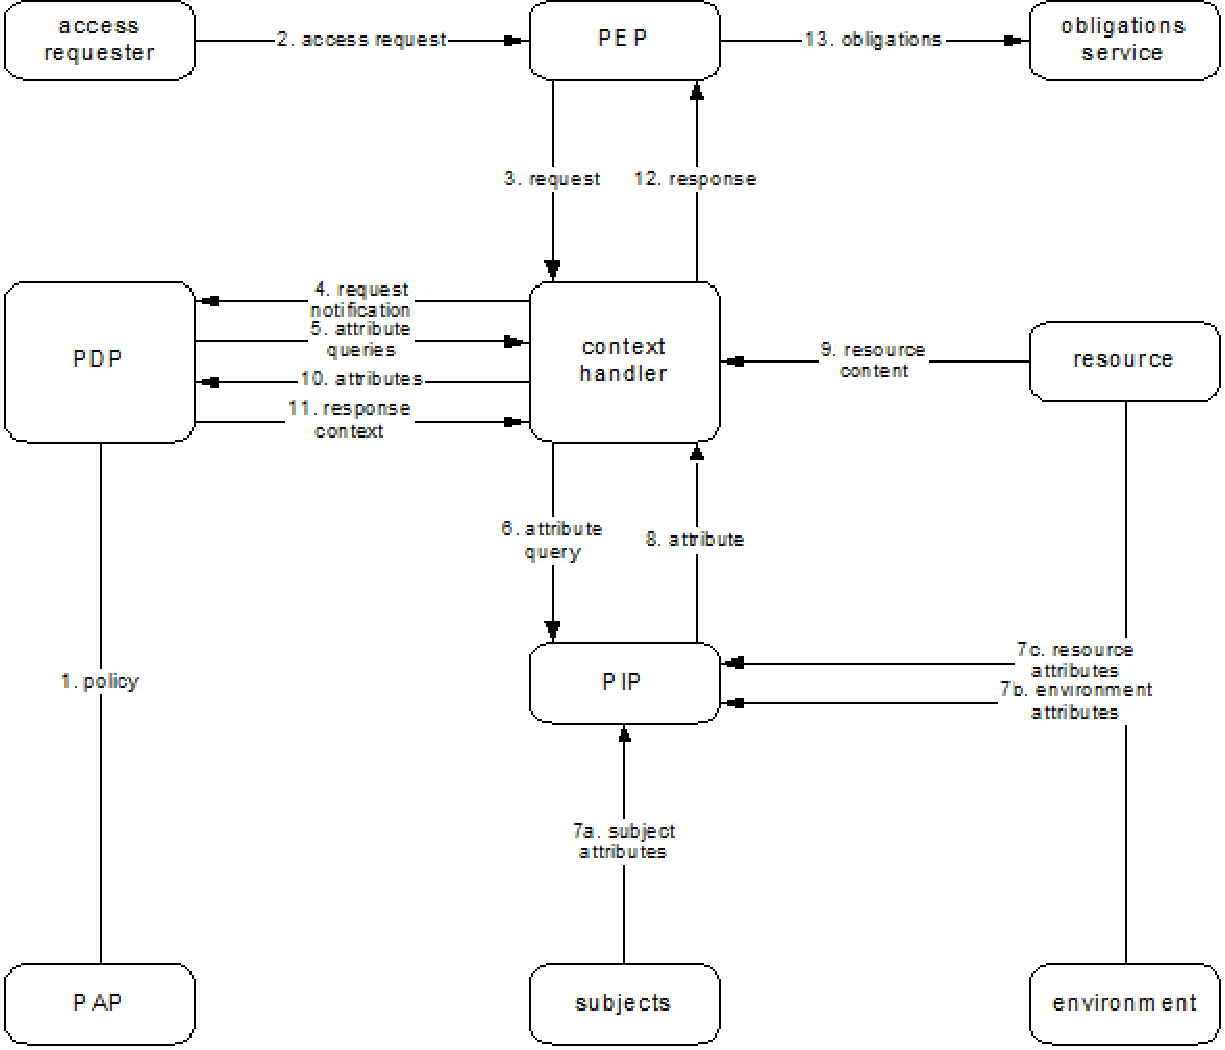
\includegraphics[scale=0.68]{it_sicherheitsmanagement/xacml.pdf}

Quelle: \url{http://docs.oasis-open.org/xacml/3.0/xacml-3.0-core-spec-os-en_files/image002.gif}



\section{IDM1 - Organisationsinternes Identitäts- und Zugriffsmanagement}
Zentrale Fragestellung: Wie können sehr viele Benutzer mit unterscheidlichen Funktionen effizient verwaltet werden?

\subsection{Identitätsspeicher}
\begin{itemize}
	\item Vorhalten digitaler Identitäten/Nutzerkonten
	\item Beispiele: HR-Systeme, Datenbanken, Verzeichnisdienste
	\item Anfragen basieren auf Eigenschaften (z.B. (L)DAP)
	\begin{itemize}
		\item \textit{Schema} bestimmt Struktur, Attribute und Matching Rules (Konsistenz wichtig!)
		\item Klassenhierarchie zur Beschreibung einer Person
	\end{itemize}
	\item Struktur Verzeichnisdienst: Hierarchisch
\end{itemize}


\subsection{Organisationsinterne Integration}

\subsubsection{Grundlegende Fragestellungen}
\begin{itemize}
	\item Identifikation der Datenquellen
	\item Datenautorität: Wem gehören die Daten?
	\item Datenaggregation: Wie werden die einer digitalen Identität zugehörigen Daten erkannt?
	\item Datenaktualität: Wie erfolgt der Abgleich?
	\item Datenkonsument: Wer benötigt welche Daten?
	\item Datenschutz
	\item Zentral vs. Dezentral und Homogenität vs. Heterogenität
\end{itemize}

\subsubsection{Bewertung zentraler Verzeichnisdienst}
\begin{itemize}
	\item Vorteile: Keine {Redundanz, komplexe Synchronisation, Inkosistenz}, Konzentration der Sicherheitsmaßnahmen an einer Stelle
	\item Nachteile: Legacy Systeme, Verlust der Autarkie, Single Point of Failure, Aggregation aller Benutzerdaten an einer Stelle (Angriffsziel)
\end{itemize}

\subsubsection{Virtual Directory}
\begin{itemize}
	\item Middleware zur dynamischen Aggregation verteilter Identitätsdaten
	\item Vorteile: Keine Redundanz, Nutzung lokaler Authentifikationsmechanismen (Pass-through Authentication)
	\item Nachteile: Verfügbarkeit zur Laufzeit nicht garantiert, keine Synchronisationsfunktionalität
\end{itemize}

\subsubsection{Meta Directory}
\begin{itemize}
	\item Synchronisation verteilter Identitätsdaten mit aggregiertem Verzeichnisdienst (vorgeschaltet)
	\item Vorteile: Sehr gute Suchperformance, Nachverfolgbarkeit von Datenflüssen
	\item Nachteile: Synchronisationsverzögerungen, zusätzliches, zentrales Berechtigungsmanagement, alle Daten zentral $\rightarrow$ Datenschutz?
\end{itemize}

\subsubsection{Provisioning System}
\begin{itemize}
	\item Anlegen, Pflege (Synchronisation), Entfernen verteilter Identitätsdaten
	\item Synchronisation verschiedener Attributwerte aus angebundenen Ressourcen nach vorgegebenen Regeln
	\item Integriertes Passwort-Management
	\item Vorteile: Self Service, Nachverfolgbarkeit von Datenflüssen
	\item Nachteile: Keine zentrale, aggregierte Sicht
\end{itemize}



\section{IDM2 - Föderatives IAM}

\subsection{Domänen-übergreifendes Identitäts- und Zugriffsmanagement}

\subsubsection{Einordnung Authentifikations- und Autorisierungsinfrastruktur (AAI)}
\begin{itemize}
	\item Auslagerung von Authentifikation und Autorisation in Infrastrukturdienste
	\item Komplexitätsreduktion (z.B. SSO)
	\item Domänenübergreifender Autausch von Identitätsdaten
	\item Nur ein Login für alle Dienste und Ressourcen benötigt
\end{itemize}

\subsubsection{Organisationsübergreifende AAI}
\begin{itemize}
	\item Voraussetzungen: Vertrauensbeziehungen zwischen den Teilnehmern, Zusammenschluss zu Föderationen
	\item Standardisierung durch Security Assertion Markup Language (SAML)
\end{itemize}


\subsection{Ausgewählte Technologien}

\subsubsection{Kerberos V4: Interrealm-Authentifikation}
\begin{itemize}
	\item Realm ist "`Herrschaftsbereich"', verlangt Namensschema zur Unterscheidung der Realms
	\item Idee: KDC von Realm B agiert wie eine Ressource in Realm A $\rightarrow$ gemeinsames Geheimnis mit KDC von Realm A
	\item Problemstellung: Vielzahl von Zugangspunkten, an allen muss authentifiziert werden
\end{itemize}

\subsubsection{RADIUS}
\begin{itemize}
	\item Problemstellung: Vielzahl von Zugangspunkten, an jedem muss authentifiziert werden
	\item Hierarchische Struktur von RADIUS Servern der verschiedenen Organisationen
	\item RADIUS Server des Network Access Servers (NAS) dient als Proxy zum RADIUS Server der Heimatorganisation (z.B. Eduroam)
	\item Authentifizierung durch die Heimatorganisation, Autorisierung durch die Zielorganisation
	\item Client und Server besitzen ein vorab vereinbartes, gemeinsames Geheimnis
	\item RADIUS verwendet keine Nachrichtenverschlüsselung
\end{itemize}

\subsubsection{SAML}
\begin{itemize}
	\item Austausch von Authentifizierungs- und Autorisierungsinformationen über institutionelle Grenzen hinweg
	\item XML basiert, OASIS Standard
	\item Bietet Profile für einige Use-cases, ist aber zusäzlich erweiterbar
	\item \textbf{Definitionen}
	\begin{itemize}
		\item Principal/Subjet: Subjekt, das Zugriff auf geschützte Ressource erhalten will
		\item Asserting Party/Identify Provider: Bietet Authentifikation von Principals
		\item Relying Party/Service Provider: Bietet Zugriff auf geschützte Ressourcen, benötigt identitätsbezogene Informationen für Autorisierungsentscheidung
	\end{itemize}
	\item \textbf{Bestandteile}
	\begin{itemize}
		\item Profiles: Definiert einen Use-case auf Basis von \textit{Bindings}, \textit{Protocols} und \textit{Assertions}
		\item Binding: Bildet SAML Protokoll auf Nachrichten- und Kommunikationsprotokolle ab
		\item Protocols: Protokolle zum Autausch von Assertions
		\item Assertions: Authentifizierungsinformationen, Attribute und Autorisierungsmerkmale
	\end{itemize}
	\item Beispielprofile: Web Browser SSO Profile, ECP Profile (SSO für nicht-browser Anwendungen), Single Logout Profile
\end{itemize}

\subsubsection{WebSSO - Ablauf}
\begin{enumerate}
	\item Weiterleitung zum Discovery Service und Auswahl des Identity Providers (optional)
	\item Weiterleitung zum IdP
	\item Authentifikation durch den IdP: Übergabe einer Assertion mit Authentication Statement und Attribute Statement
	\item Weiterleitung zum Service Provider und Übergabe der Assertion
\end{enumerate}
Bindings: HTTP-Redirect, HTTP Post

\subsubsection{SAML in der Praxis: Shibboleth}
\begin{itemize}
	\item OpenSource (Apache License)
	\item Attribute Based Access Control
	\item Ermöglicht föderatives Identitätsmanagement
	\item Einstz beispielsweise bei Elsevier, Asknet, Gigamove
	\item \textbf{Ablauf am Beispiel Gigamove}
	\begin{enumerate}
		\item Aufruf der Gigamove Webseite der RWTH Aachen
		\item Weiterleitung zum DFN, Heimateinrichtung auswählen
		\item Weiterleitung zum Shibboleth Provider des KIT
		\item Weiterleitung "`zurück"' zur Gigamove-Webseite der RWTH Aachen
	\end{enumerate}
\end{itemize}

\subsubsection{Zugang über einen SSH-Server}
Es existieren drei Varianten.
\begin{enumerate}
	\item \textbf{Variabte 1 - Enhanced Proxy}
	\begin{itemize}
		\item Delegation der Autorisierungsentscheidung über PAM
		\item Vorteil: Kein spezieller SSH-Client nötig
		\item Nachteil: Password wird im Klartext an den Service Provider übertragen
	\end{itemize}
	\item \textbf{Variabte 2 - Enhanced Client}
	\begin{itemize}
		\item PAM dient lediglich als Schnittstelle zum SAML-SP
		\item SSH-Client fungiert als Enhanced Client
		\item Vorteil: Service Provider erhält keine Kenntnis des Passworts
		\item Nachteil: Modifizierter SSH-Client nötig
	\end{itemize}
	\item \textbf{Variabte 3 - Public Key based Authentication}
	\begin{itemize}
		\item Authentifizierung gegen Service Provider
		\item Autorisierung basiert auf aktuellen Attributen des Identity Providers
		\item PAM beauftragt SAML-SP eine AttributeQuery durchzuführen
	\end{itemize}
\end{enumerate}

\subsubsection{Metadatenverwaltung der Föderation}
\begin{itemize}
	\item Es muss sichergestellt werden, dass alle Föderationsmitglieder sich gegenseitig authentifizieren können $\rightarrow$ Metadaten zur Definition der Föderation notwendig
	\item Metadaten können zentral in einem Dokument verwaltet werden, enthalten Zertifikate der SPs und IdPs und enthalten Adressen der unterstützten Kommunikationsschnittstellen der Teilnehmer
\end{itemize}


\subsection{Föderatives Identitätsmanagement im Web 2.0}

\subsubsection{OAuth 1.0}
\begin{itemize}
	\item Anwendungsfall: Benuter (User) kann einer Anwendung (Consumer) Zugriff auf Daten erlauben, die von einer anderen Anwendung verwaltet werden (Service Provider)
	\item \textbf{Ablauf}
	\begin{enumerate}
		\item User stellt Anfrage an den Consumer
		\item Consumer beantragt ein Abfrage-Token beim Service-Provider
		\item User wird zum Service Provider weitergeleitet
		\item User gibt seine Daten und bestätigt die Anfrage des Consumers
		\item Consumer erhält Zugangs-Token
		\item Consumer kann auf die geschützten Ressourcen zugreifen
	\end{enumerate}
\end{itemize}

\subsubsection{OAuth 2.0}
\begin{itemize}
	\item Weiterentwicklung von OAuth 1.0, allerdings nicht rückwärtskompatibel
	\item Fokus auf Komplexitätsreduktion für den Client(-entwickler)
\end{itemize}

\subsubsection{OpenID}
\begin{itemize}
	\item \textbf{Ablauf}
	\begin{enumerate}
		\item Nutzer gibt seine OpenID-URL an
		\item SP lädt diese URL herunter, darin enthalten: Verweis auf den IdP
		\item Optional: RP handelt mit IdP (per Diffie-Hellman) einen gemeinsamen Schlüssel aus
		\item SP schickt einen HTTP-Redirect auf den IdP an den Nutzer
		\item Nutzer authentifiziert sich beim IdP
		\item IdP schickt HTTP-Redirect an den SP mit Aussage über die Authentifizierung
		\item SP prüft die Aussage. Falls DH-Schlüssel vorhanden hiermit, anderenfalls durch Nachfrage
	\end{enumerate}
	\item Bewertung: Massive Verbreitung, allerdings keine Verschlüsselung gefordert, Nutzer kann eine beliebige Id angeben, die gemäß Verfahren heruntergeladen werden muss
\end{itemize}


\subsection{Zusammenfassung}
\begin{itemize}
	\item Föderatives Identitätsmanagement erlaubt einen organisationsübergreifenden Austausch von Identitätsinformationen
	\item Vorteile: Aktualität, SSO, viele Registrierungsprozesse entfallen
	\item Allerdings organisationsübergreifendes Vertrauen notwendig
\end{itemize}



\section{Business Continuity Management}

\subsection{Motivation}
\begin{itemize}
	\item Unternehmen sind abhängig von Einrichtungen, Rechnern, Diensten, Personal, Daten, Kommunikationsverbindungen, etc.
	\item Was passiert, wenn diese Ressourcen im Krisenfall ausfallen?
\end{itemize}


\subsection{Was ist Business Continuity Management}
"`Ganzheitlicher Managementprozess zur Fortführung der kritischen Geschäftsprozesse bei Eintritt eines Notfalls."'\footnote{BSI-Standard 100-4, S. 100}

\subsubsection{Notfallmanagement nach BSI 100-4}
\begin{enumerate}
	\item Initiierung durch das Management mit Zieldefinition und Organisation der Verantwortlichkeiten und des Krisenstabs
	\item Konzeptions des Notfallvorsorgekonzepts mit \textit{Business Impact Analyse} (Priorisierung der Geschäftsprozesse für den Krisenfalls), Risikoanalyse und der Erstellung eines Notfallhandbuchs
	\item Umsetzung des Notfallvorsorgekonzepts: Kosten- und Aufwandschätzung, Umsetzung der Maßnahmen, Sensibilisierung und Schulung
	\item \textbf{Notfallbewältigung}
	\begin{enumerate}
		\item Meldung bei zentraler Meldestelle
		\item Eskalation durch Krisenstabsleiter. Störung/Notfall/Krise?
		\item Sofortmaßnahmen einleiten
		\item Notfall bewältigen: Do-Plan-Check-Act
	\end{enumerate}
	\item Tests und Übungen: Tests der wesentlichen Bestandteile, Angemessen beachten
	\item Aufrechterhaltung und Verbesserungen: Regelmäßige Bewertung des Notfallmanagements
\end{enumerate}
Iterativer Prozess, daher im Anschluss ein Sprung zu (2).

\subsubsection{Business Impact Analyse}
\begin{enumerate}
	\item Auswahl einzubeziehender Organisationseinheiten und Prozesse
	\item Schadensanalyse
	\item Festlegung Wiederanlaufparameter
	\item Priorisierung der Geschäftsprozesse
	\item Abschätzung des Ressourcenbedarfs
	\item Priorisierung der Ressourcen
\end{enumerate}

\subsubsection{Notfallhandbuch}
Das Notfallhandbuch besteht üblicherweise aus folgenden Teilen:
\begin{itemize}
	\item Sofortmaßnahmen
	\item Krisenstabsleitfaden
	\item Krisenkommunikationsplan
	\item Geschäftsfortführungsplan
	\item Wiederanlaufplan
\end{itemize}


\subsection{Vorfallbehandlung}

\subsubsection{Computer Emergency Response Team (CERT)}
\begin{itemize}
	\item Lösung konkreter Sicherheitsvorfälle
	\item Warnungen vor Sicherheitslücken mit Lösungsansätzen
	\item Verschiedene CERTs, die verschiedenen Einrichtungen zugeordnet sind (z.B. Bund oder KIT)
\end{itemize}



\section{Secure Data Outsourcing}

\subsubsection{Generelle Vorteile}
\begin{itemize}
	\item Kosten sparen
	\item Höhere Verfügbarkeit/Robustheit
	\item Vereinfachte Administration
	\item Nachteil: Mangelnde Datenvertraulichkeit. Naheliegend: Verschlüsselung, lässt allerdings dann auch keine Datenverarbeitung vor Ort zu (Anbieter ist "`Honest, but curious"')
\end{itemize}


\subsection{Existierende Ansätze}

\subsubsection{Cryptografische Maßnahmen}
\begin{itemize}
	\item Deterministische Verschlüsselung: Ermittlung einzelner Chiffrate ohne Schlüssel schwierig, allerdings sind Chiffrate unterscheidbar
	\item Probabilistische Verschlüsselung: Chiffrate weder lesebar noch unterscheidbar. Jedoch keine Anfragen möglich
	\item Homomorphe Verschlüsselung: $Enc(k_1) \oplus Enc(k_2) = Enc(k_1 \otimes k_2)$. Ermöglicht Aggregation von Attributwerten, allerdings hoher Rechenaufwand und keine SELECT-Anfragen möglich
\end{itemize}

\subsubsection{Data Partitioning}
\begin{itemize}
	\item Aufteilung der Daten auf verschiedene Storage Provider $\rightarrow$ Unkenntlichkeit von Zusammenhängen zwischen Attributen
	\item Nachteil: Mehrere Storage Provider notwendig; ggf. zu wenige vorhanden
\end{itemize}

\subsubsection{k-Anonymisierung}
Jede mögliche Belegung eines Identifikators muss entweder nicht oder mindestens k-mal im Datensatz vorkommen. Operationen zur Sicherstellung: Suppresion (*), Generalization (M*) oder Einfügen falsche Einträge.


\subsection{Aktuelle Forschung: Securus}
Anwendungsfall: Datenbank mit Patientendaten.

\subsubsection{Von Securus adressierte Schutzziele}
\begin{itemize}
	\item Vertraulichkeit: Sicherstellung der Vertraulichkeit von Daten, die bei externen Providern abgelegt werden
	\item Datenschutz: Datenschutzrechtliche Vorgeben werden wahrgenommen und erfüllt
	\item Verfügbarkeit: Auslagern von Daten ermöglicht eine Steigerung der Verfügbarkeit der Daten
\end{itemize}

\subsubsection{Workflow}
\begin{enumerate}
	\item Benutzerseite: Definition des \textit{Policy Profile} über \textit{Securus Latin} (domänenspezifische Sprache)
	\item Securus: Tranformiere \textit{Policy Profile} in den \textit{Mediator}
	\item Mediator: \textit{Mediator} übernimmt die Verwaltung der Storage Provider und leitet alle Anfragen weiter
\end{enumerate}

\subsubsection{Access Policies} 
Access Policies spezifizieren eine Menge von Anfragen, die effizient auf den Daten ausführbar sein sollen.

\subsubsection{Confidential Constraits (CCs)}
Eine Untermenge an Attributen, deren Kombination als vertraulich gilt.

\subsubsection{Inference Constraits (ICs)}
Es wird angenommen, dass Angreifer kein Wissen aus deterministischen Chiffraten des entsprechenden Attributs gewinnen können.

\subsubsection{Securus-PT: Transformation des Policy Profiles}
\begin{enumerate}
	\item Verschlüssele jeden Wert der \textit{data table}. Einträge können per Id abgerufen werden, es können jedoch keine Anfragen ausgeführt werden
	\item Erstelle \textit{index table} für jede Access Policy. Ermöglicht effiziente Ausführung von entsprechenden Anfragen, die Attribute/Kombinationen aus Attributen werden per Id angesprochen
	\item \textbf{Substitutionsklassen}
	\begin{itemize}
		\item Idee: Klassifikation der Sicherheitsmechanismen anhand der Art, wie Attributwerte beim Storage Provider vorliegen
		\item Confidential Constraits und Access Policies schränken die Möglichkeiten ein, Substitutionsklassen zu wählen $\rightarrow$ Lösung als Integer Linear Programming von einem ILP-Server
		\item Beispiel: Mitarbeiterdatenbank, verteilt auf zwei Storage Provider. Name, DoB und Salary
		\begin{enumerate}
			\item Verschlüssele jeden Wert der \textit{data table}
			\item Erstelle \textit{index table} für jede Access Policy: Effiziente Abfragen möglich. Alle \textit{index tables} werden bei allen Storage Providern angelegt, bleiben allerdings ggf. leer
			\item Fülle \textit{index tables}, so dass alle ICs und CCs erfüllt sind mit (un-)verschlüsselten Werten
		\end{enumerate}
	\end{itemize}
\end{enumerate}

\subsubsection{Zusammenfassung Securus}
\begin{itemize}
	\item \textbf{Konzept}
	\begin{itemize}
		\item Herausforderung für sicheres Data Outsourcing: Matching von Datenvertraulichkeits- und Datenanfragbarkeitsanforderungen
		\item Securus automatisiert diesen Prozess
	\end{itemize}
	\item \textbf{Benutzung}
	\begin{enumerate}
		\item Definition von Access Policies und Confidential Constraits mit Securus-Latin
		\item Nutzung von generierten Mediatoren zur Ablage und Abfrage von Daten
	\end{enumerate}
	\item \textbf{Funktionsweise}
	\begin{itemize}
		\item Securus transformiert Policies in ein ILP-Problem
		\item Die eingesetzten Sicherheitsmechanismen werden dann entsprechend gewählt
	\end{itemize}
\end{itemize}



\section{Secure Data Sharing}

\subsection{Problemstellung}
\begin{itemize}
	\item Vorteile: Verfügbarkeit, Bandbreite, vereinfachte Administration
	\item Im Gegensatz zu \textit{Data Outsourcing} ist Teilen der Daten explizite Anforderung
	\item Nachteil: Vertraulichkeit und Integrität der Daten gefährdet
\end{itemize}

\subsubsection{Verschlüsselung der Daten}
\begin{itemize}
	\item Naiver Ansatz: Daten symmetrisch verschlüsseln und Datenschlüssel direkt an andere weitergeben. Nachteile: Entzug von Zugriffsrechten aufwendig, sicherer Kanal zur Schlüsselweitergabe nötig
	\item Besser: Austausch neuer Schlüssel durch Nutzung bereits ausgetauschter Schlüssel. Initialer Austausch von (a-)symmetrischen Schlüsseln notwendig
\end{itemize}


\subsection{Shared Cryptographic File Systems}
\begin{itemize}
	\item Vertraulicher Datenaustausch zwischen Benutzern über externe Speicheranbieter mit Ende-zu-Ende-Sicherheit
	\item Zusätzlich zur Sicherung der Integrität: Signaturen und/oder MACs
	\item Initialer Autausch nicht Teil des SCFS
\end{itemize}

\subsubsection{SiRiUS}
\begin{itemize}
	\item Stellt Vertraulichkeit und Integrität sicher: Nutzerdaten werden vor Ablage auf dem Dateiserver verschlüsselt und signiert
	\item Jeder Benutzer besitzt ein Schlüsselpaar
	\item Ein Besitzer für jeden Verzeichnisbaum
	\item Overlays zu bestehenden Dateisystemen
	\item Pro Datei ein symmetrischer Verschlüsselungskey und ein Keypair zur Signierung
	\item Lesezugriff durch Weitergabe des sym. Schlüssels und Schreibzugriff durch Weitergabe des privaten Schlüssels
	\item Sicherung der Metadaten: Besitzer der Datei signiert jede Änderung mit seinem privaten Schlüssel. Problem: Freshness nicht gewährleistet (Rollback-Angriff: Ehemals Schreibberechtigte können ältere md-Files hochladen, um Schreibberechtigung wieder zu erlangen. Gegenmaßnahmen: Gültigkeit der Signatur periosdisch auffrischen, resscourcenintensiv, Stichwort Hash-Tree)
	\item Beim Entzug von Leserechten: Sofortige Neuverschlüsselung
\end{itemize}

\subsubsection{Cepheus}
\begin{itemize}
	\item Stellt ebenfalls Vertraulichkeit und Integrität der Nutzerdaten sicher
	\item Führt zusätzliche Schlüssel für Benutzergruppen ein
	\item Keine Unterscheidung zwischen Lese- und Schreibrechten
	\item Sicherung der Integrität und Freshness der Metadaten über \textit{Merkle Hash Tree}
	\item Beim Entzug von Leseberechtigung: Lazy Revocation (Problem: Entzug erst nach Neuschreiben der Daten wirksam)
\end{itemize}

\subsubsection{Cryptree}
\begin{itemize}
	\item Ordnet jeder Datei/Verzeichnis einen Satz Schlüsseln zu
	\item Eigener \textit{Write Cryptree} für das Erteilen von Schreibrechten, Dateien werden zusätzlich signiert
	\item Setzt ebenfalls Lazy Revocation ein
\end{itemize}

\subsubsection{Shared Cryptographic File Systems: Risiko}
Tradeoff zwischen Verminderung des Risikos gegenüber Kosten/Ressourcenbedarf.


\subsection{Abstrakte Repräsentation: Schlüsselgraph}
\begin{itemize}
	\item Benutzer und deren bekannte Schlüssel bilden einen Schlüsselgraphen
	\item Erweiterung: Verschlüsselte Ressourcen
	\item Systeme für Secure Datasharing erzeugen implizit einen Schlüsselgraphen
	\item Ziel: Veringere Anzahl der Kanten
	\item Simpler Ansatz, abgeleitet aus Zugriffskontrollmatrix: Ein Schlüssel pro Benutzer und pro Ressource
	\item Mögliche Optimierung: Capability List, benötigt je nach Szenario weniger Kanten $\rightarrow$ welcher Ansatz ressourcenschonender ist, hängt vom Szenario ab
\end{itemize}


\subsection{Aktuelle Forschung: Abschätzen des Ressourcenbedarfs über Änderungen des Schlüsselgraphen}
\begin{itemize}
	\item Ziel: Abhängigkeit des Ressourcenbedarfs von konkretem Szenario und konkretem System für Secure Data Sharing finden
	\item Vorgehen: Modellierung des Systems als Regelsatz, der Änderungen am Schlüsselgraphen vornimmt, dann Ableitung des Ressourcenbedarfs aus den Änderungen am Schlüsselgraphen $\rightarrow$ Eingabe für Simulation: Workloads als Abfolge von Ereignissen (Erfassung realistischer Workloads schwierig)
\end{itemize}



\section{Anonymität}
\begin{itemize}
	\item ... kann Vertraulichkeit "`ersetzen"'
	\item ... kann Datenschutz ermöglichen
	\item ... kann Voraussetzung für ein technisches System sein
	\item ... kann vor Repressalien schützen, bietet aber auch Missbrauchspotential
\end{itemize}

\subsubsection{Definition nach BSI:}
Die Identität einer oder mehrerer an einem anonymen Vorgang beteiligter Instanzen ist nicht bestimmbar, weil sie entweder
\begin{itemize}
	\item den anderen beteiligten Instanzen nicht bekannt ist (Nichtbewusstsein),
	\item gegenüber den anderen beteiligten Instanzen nicht in Erscheinung tritt (Nichtgenanntsein) \\ oder
	\item innerhalb des anonymen Vorgangs ohne erkannbaren Namen agiert (Namenlosigkeit).
\end{itemize}
\footnote{\url{https://www.bsi.bund.de/DE/Publikationen/Studien/anonym/wasistanonymitaet.html}}

Problem: Identität mit hinreichend großem Aufwand eben doch bestimmbar, besonders im IT-Umfeld.

\subsubsection{Anwendungsfelder}
\begin{itemize}
	\item Anonymisierung von Daten
	\item Anonyme Kommunikation (Schwerpunkt in dieser Vorlesung)
\end{itemize}

\subsubsection{Pseudonymisierung}
\begin{itemize}
	\item Erlaubt eine digitale Identität zu verwenden ohne seine reale Identität preiszugeben. Enscheidung, welche Informationen er über sich herausgiebt, liegt beim Subjekt selbst
\end{itemize}

\subsubsection{Anynome Kommunikationsstufen}
Eigenschaften anonymer Kommunikation: Sender- und Empfängeranonymität.
\begin{enumerate}
	\item Absolute anonymity: Beobachter kann nicht feststellen, ob eine Nachricht verschickt wurde.
	\item Beyond suspicion: Beobachter kann nicht feststellen, von wem die Nachricht verschickt wurde
	\item Probable innocence: Für den Beobachter ist es wahrscheinlicher, dass die Nachricht nicht vom Sender kommt, als dass die von ihm kommt
	\item Possible innocence: Für Beobachter exisitiert Wahrscheinlichkeit, dass die Nachricht nicht vom Sender kommt
	\item Exposed: Beobachter kann Sender identifizieren, aber gegenüber Dritten nicht beweisen, dass der Sender sie wirklich gesendt hat
	\item Provably exposed: Verbindlichkeit ist gegeben
\end{enumerate}

\subsubsection{Anonymität im Internet}
\begin{itemize}
	\item Szenario: Anonymes Senden von Nachrichten über (vertrauenswürdigen) Proxy
	\item Erweiterung: Einführen mehrerer Proxies in Reihe (Mix-Kaskaden). Problem: Mögliche Kollaboration zwischen Mixes $\rightarrow$ Mixes dynamisch wählen
	\item \textbf{Onion Routing}
	\begin{itemize}
		\item Dynamische Wahl der Mixes, Benutzer können eigenen Endknoten als Mix anbieten und mischen eigenen Traffic und den Traffic der anderer Knoten.
		\item Mögliches Problem, Sybil-Attacke: Beobachten von Kommunikationsmuster im Netz
		\item Implementierungen: Tor, Freenet, I2P
	\end{itemize}
\end{itemize}



\section{Peer-to-Peer und Online Social Networks}

\subsection{Methodik für empirische OSN-Studien}
\begin{itemize}
	\item Datenschutzkonforme und Privatsphäre-wahrende Analyse: Analyse vollständig zur Laufzeit des Analyse-Systems, ledigliches Speichern statistischer (anonymisierter) Daten
	\item Breitensuche: Analysiere mind. ein Profil und davon ausgehend alle Freunde, etc.
	\item Tiefensuche: Analysiere ein Seed-Profil, dann einen Freund, dann einen Freund des Freunde, etc.
\end{itemize}


\subsection{Online Social Networks}
\begin{itemize}
	\item Attribut-Verfügbarkeit. Mögliche Gefahr: Wenn diverse OSN-Profile eines Nutzer in Verbindung gebracht werden, kann ein umfassendes digitales Abbild der Person erstellt werden (Freundeslisten zu ca. 50\% öffentlich verfübar)
	\item Profil-Verknüpfbarkeit (Linkability)
	\item \textbf{Attribut-Vorhersagbarkeit (Attribute Prediction)}
	\begin{itemize}
		\item Freundeslisten in ca. 50\% der Profile öffentlich
		\item >78\% teilen mindestens ein Attribut öffentlich, dass sie auch verstecken könnten
		\item Hohe Genauigkeit bei Attribut-Vorhersagen
	\end{itemize}
\end{itemize}


\subsection{Zusammenfassung}
\begin{itemize}
	\item \textbf{Attributverfügbarkeit}
	\begin{itemize}
		\item Viele Attribute noch immer öffentlich verfügbar
		\item Alt-Profile oft noch online
		\item Ca. die Hälfte der Freundeslisten öffentlich
	\end{itemize}
	\item \textbf{Quantifizierte Risiken}
	\begin{itemize}
		\item Linkability: Vier überlappende Freunde oft ausreichend für Linking
		\item \textbf{Attribute Prediction}
		\begin{itemize}
			\item Location-Attribute und Alter kann predeziert werden (mit Ungenauigkeit)
			\item Andere Attribute schwerer zu prezidieren, wenn kein komplexer Algorithmus oder zusätzliche Informationen hinzugezogen werden
		\end{itemize}
	\end{itemize}
\end{itemize}
